\documentclass[tikz, border=2pt]{standalone}
\usepackage{tikz}
\usepackage{pgfplots}
\usetikzlibrary{decorations.pathreplacing,calc}
\begin{document}
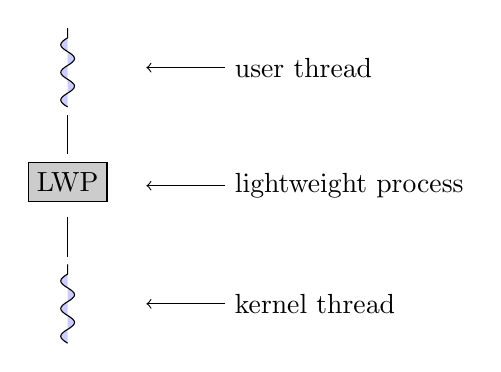
\begin{tikzpicture}
    \foreach \y in {0,3}
    {
        \draw [fill=blue!20, decorate, decoration={coil,aspect=0}] (0,\y) -- (0,\y+1);
    }
    \foreach \y in {1.1, 2.4}
    {
        \draw (0,\y) -- (0,\y+0.5);
    }
    \draw [fill=black!20] (-0.5,1.8) rectangle (0.5,2.3);
    \node [align=center] at (0,2.05) {LWP};
    \foreach \y in {0.5,2,3.5}
    {
        \draw [->] (2,\y) -- (1,\y);
    }
    \node [align=left, right] at (2,0.5) {kernel thread};
    \node [align=left, right] at (2,2) {lightweight process};
    \node [align=left, right] at (2,3.5) {user thread};
\end{tikzpicture}
\end{document}